\begin{figure}
    \centering
    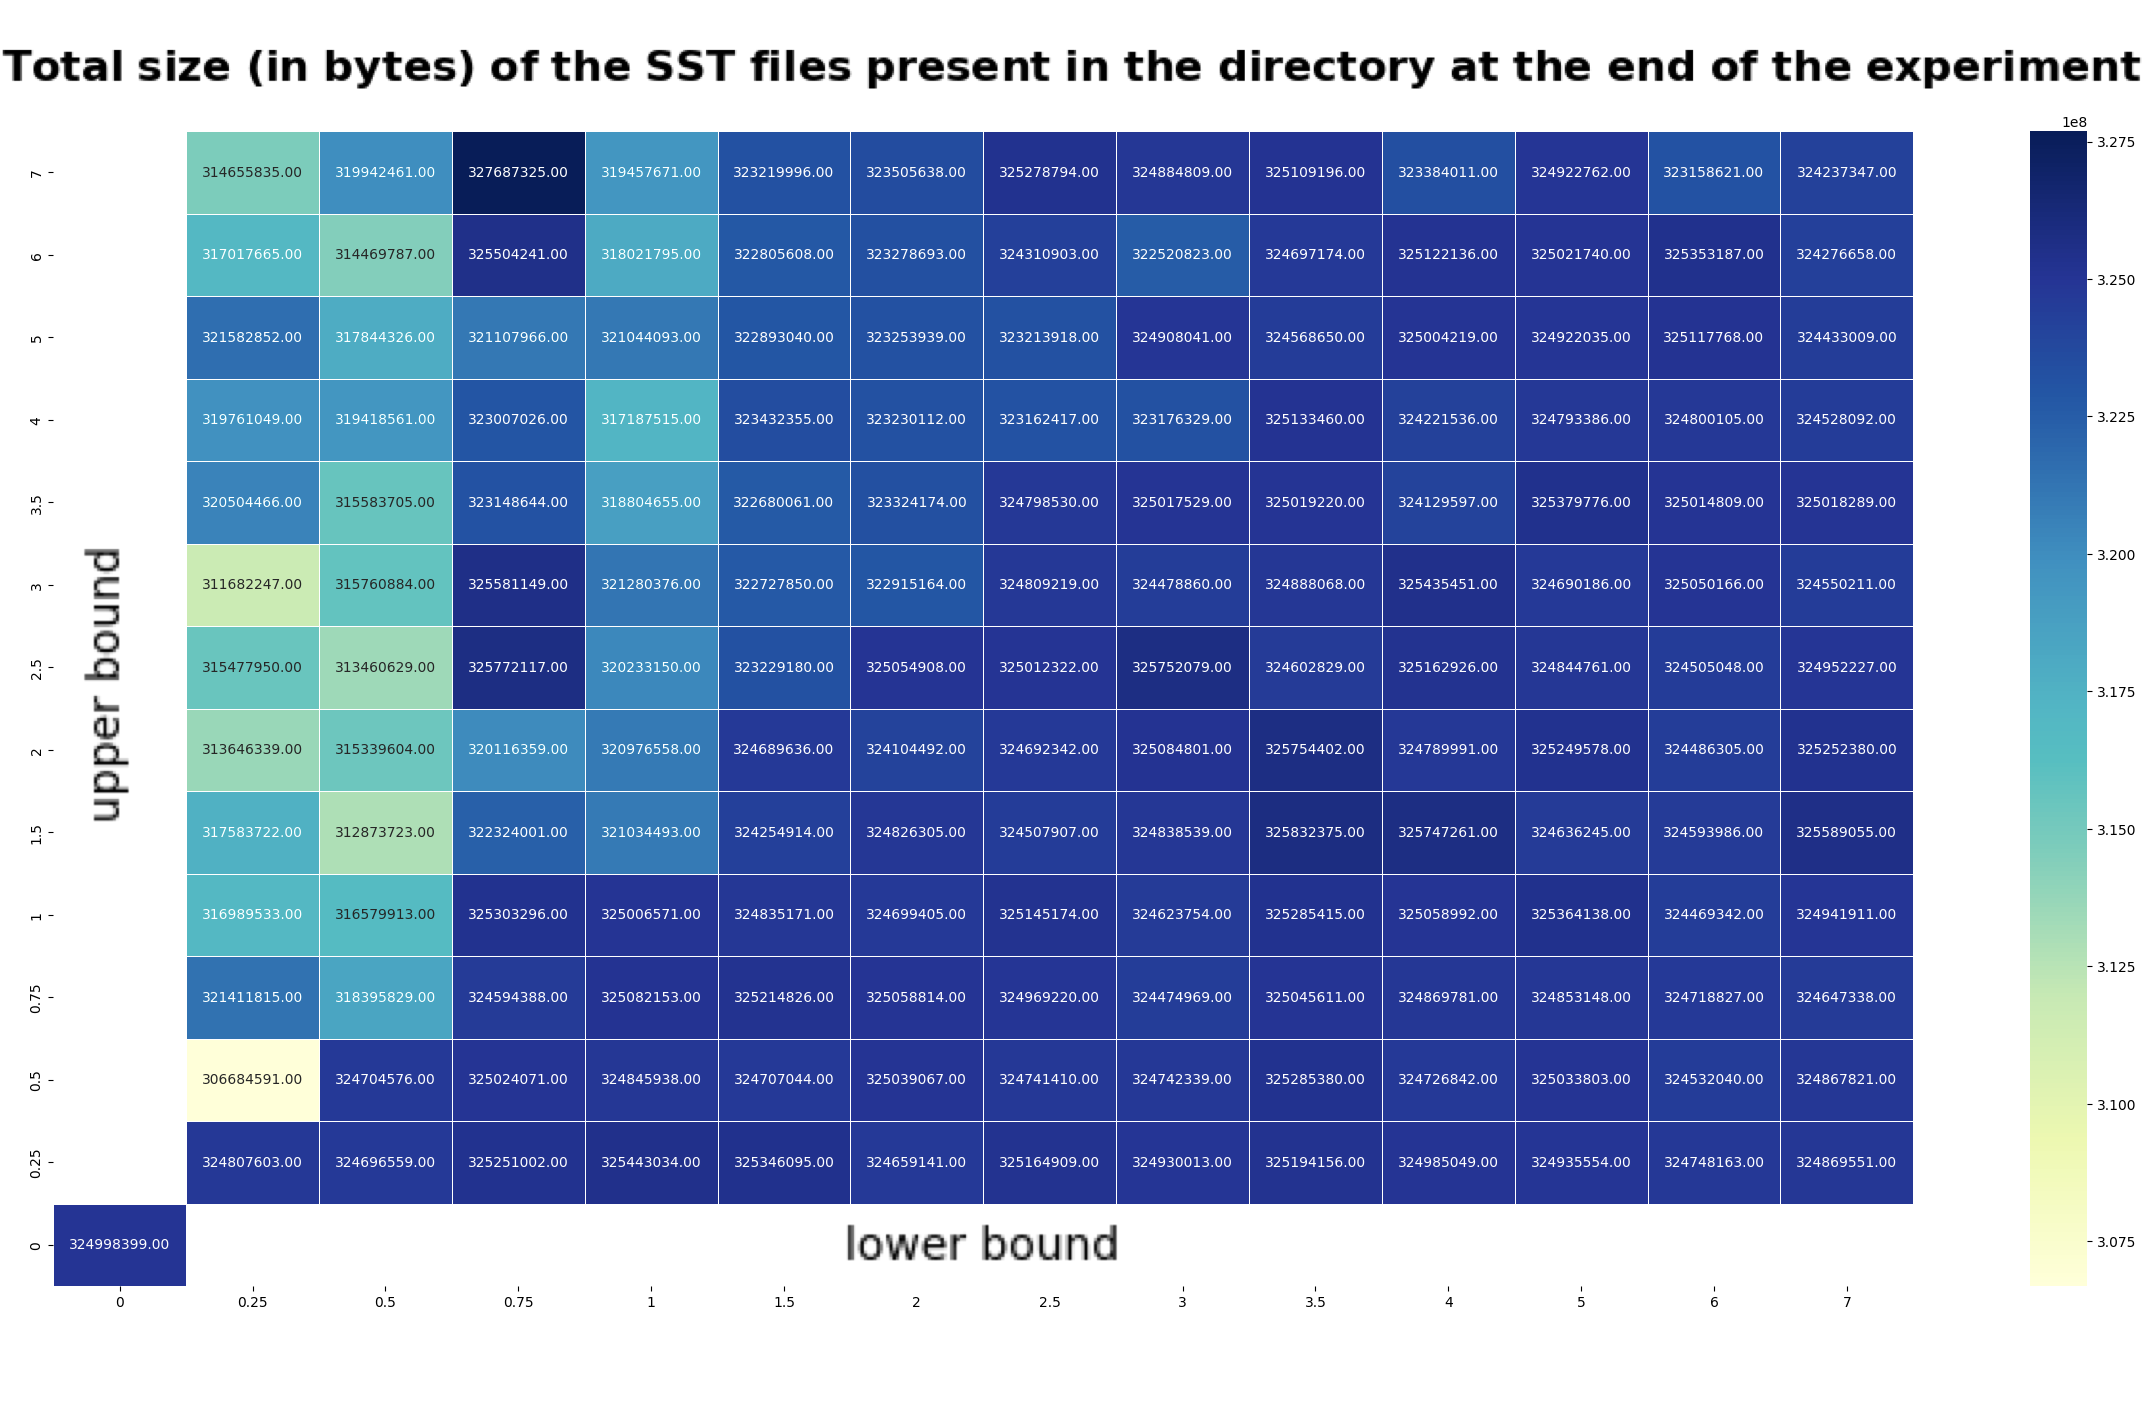
\includegraphics[width=\linewidth]{Figures/size-of-database.png}
    \caption{Figure shows how the size of database changes with different values of lower bound and upper bound.
    The horizontal axis shows the lower bound and vertical shows the upper bound. The left bottom corner shows the 
    Vanilla and rest all are for RQDC.}\label{fig:db_size_for_different_ub_lb}
\end{figure}

\begin{figure}
    \centering
    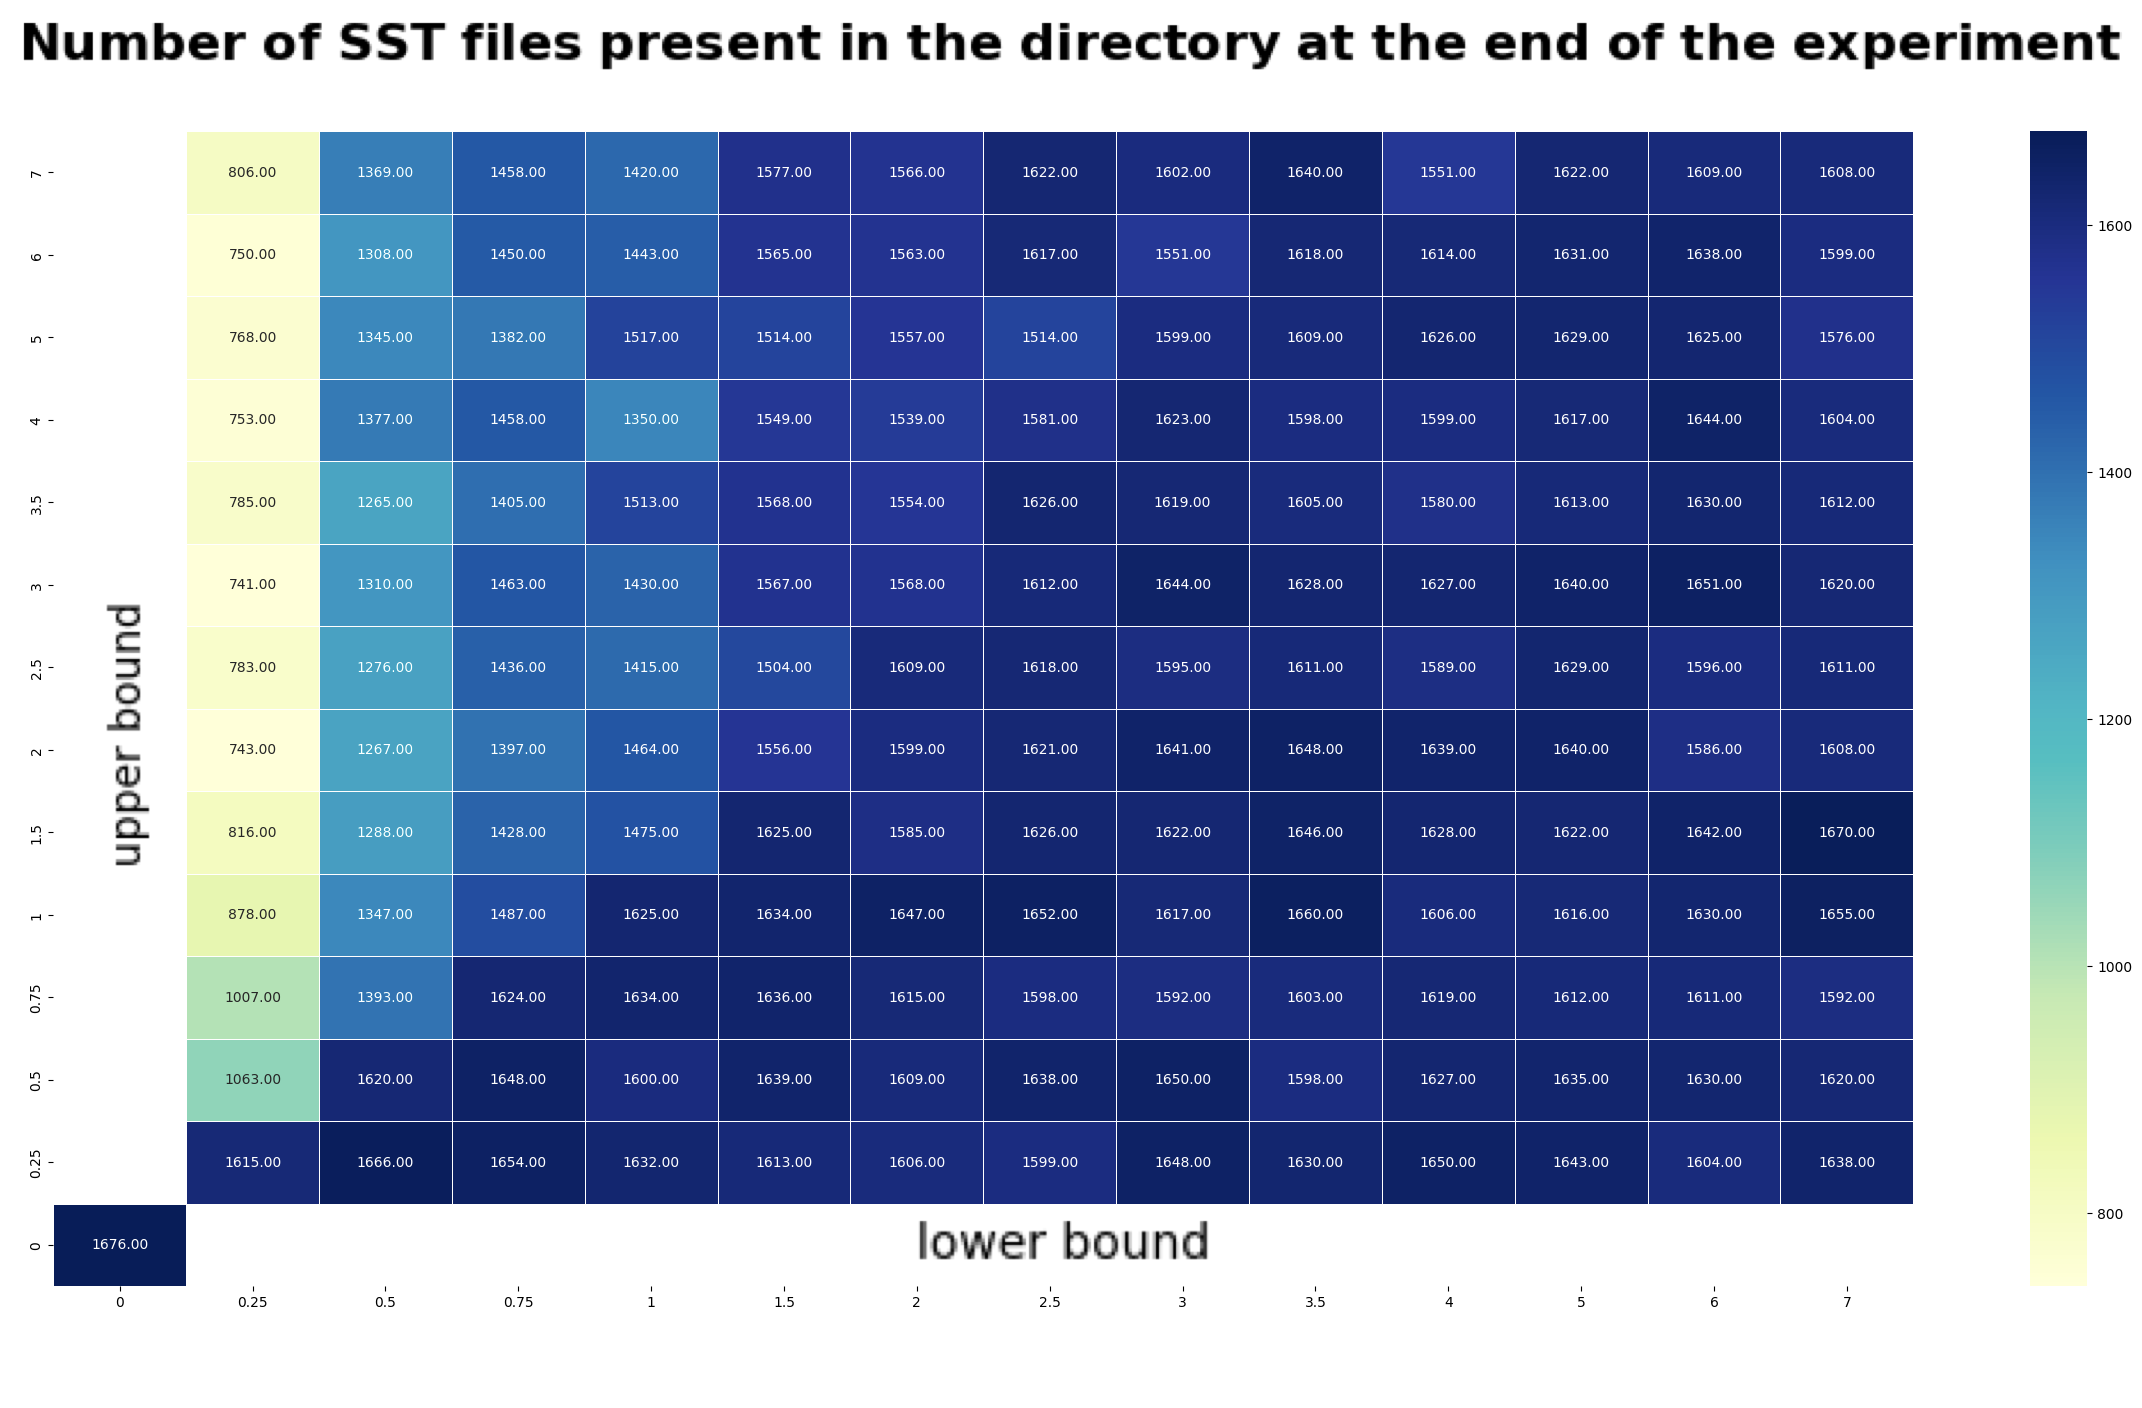
\includegraphics[width=\linewidth]{Figures/number-of-sst-files.png}
    \caption{Figure shows how the number of SST files changes with different values of lower bound and upper bound.
    The horizontal axis shows the lower bound and vertical shows the upper bound. The left bottom corner shows the 
    Vanilla and rest all are for RQDC.}\label{fig:number_of_sst_files_ub_lb}
\end{figure}

\begin{figure}
    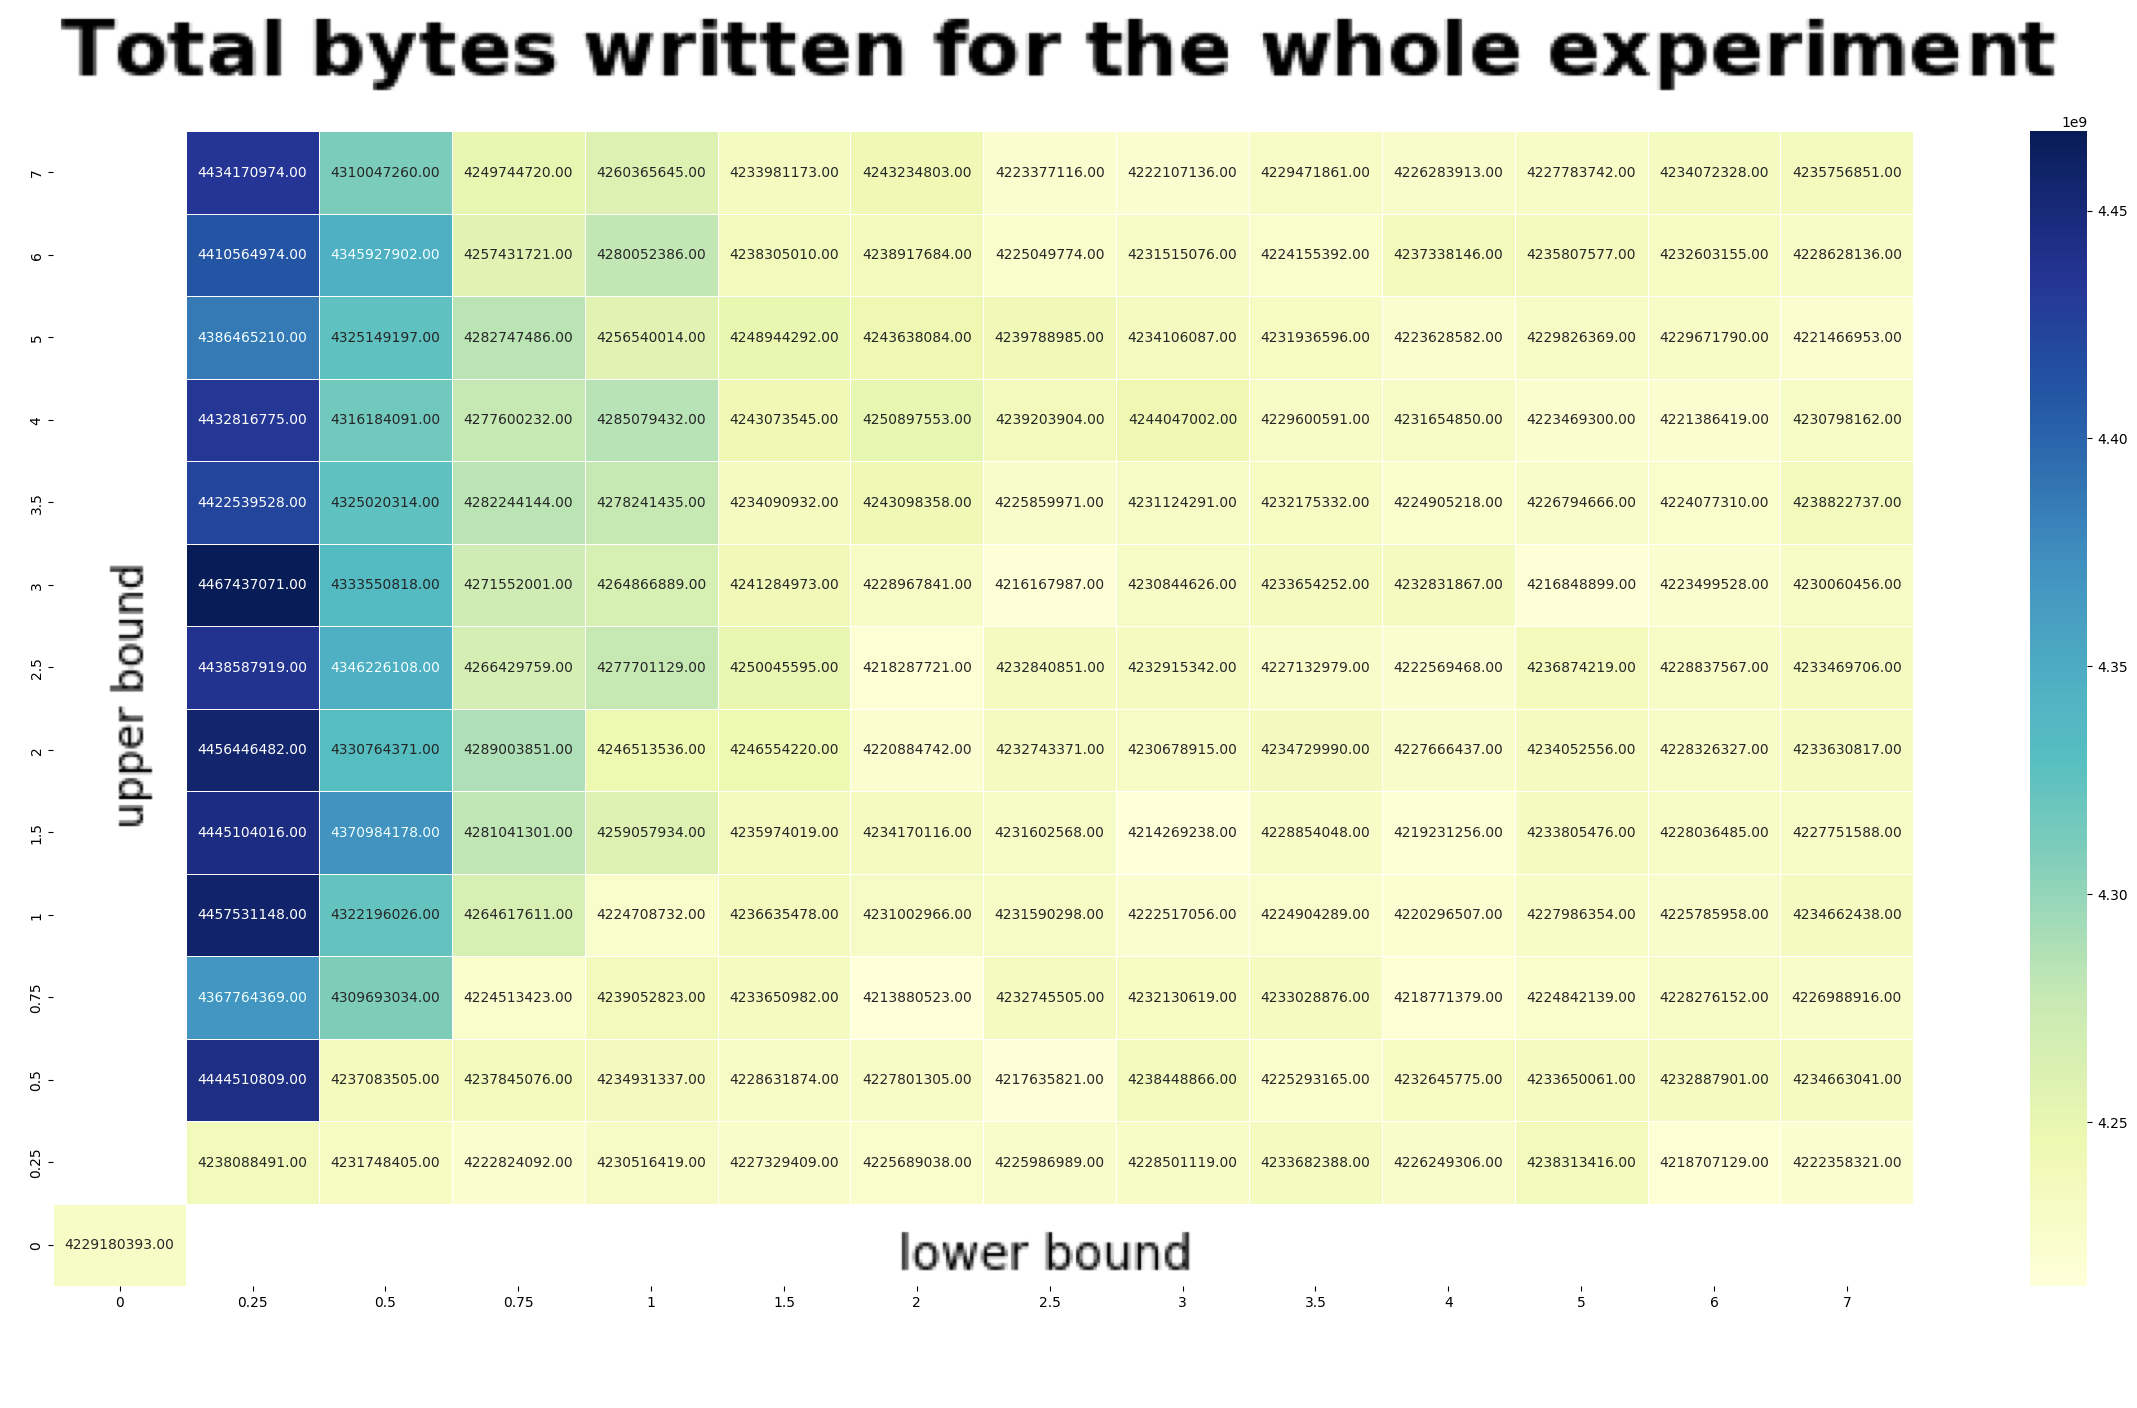
\includegraphics[width=\linewidth]{Figures/total_bytes_written.png}
    \caption{Figure shows the total number of bytes written for the execution of whole workload using different lower 
    and upper bound thresholds. The left bottom corner shows the Vanilla and rest all are for RQDC.}
\end{figure}

\begin{figure}
    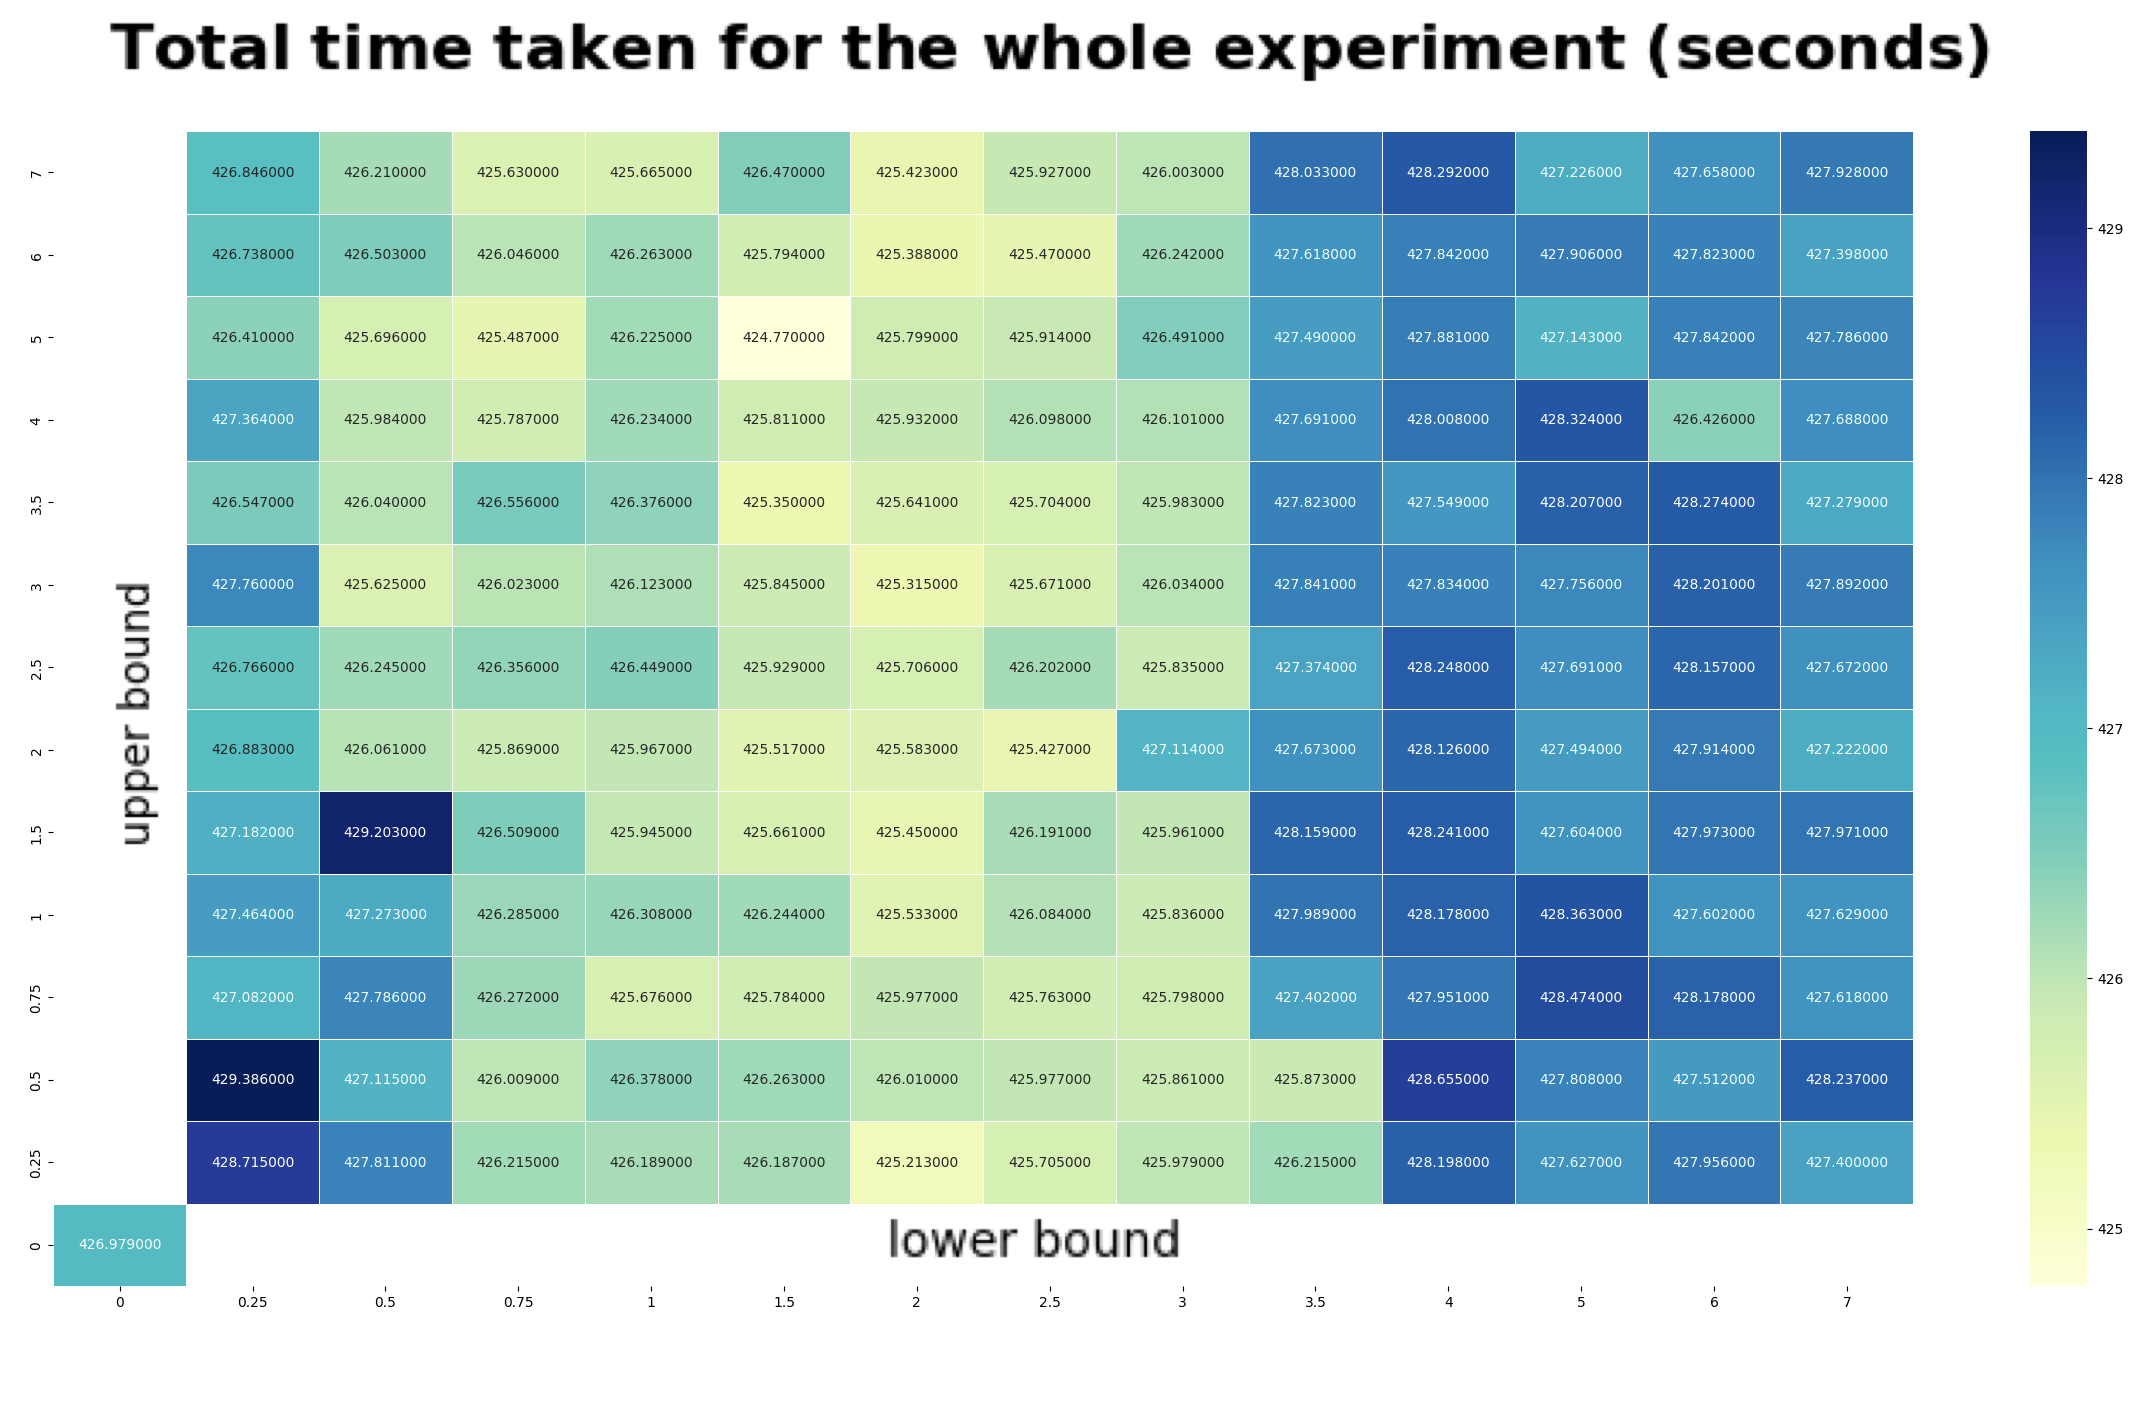
\includegraphics[width=\linewidth]{Figures/total_time_taken.png}
    \caption{Figure shows the change in workload execution time for different lower and upper bound values. The left 
    bottom corner shows the Vanilla and rest all are for RQDC.}
\end{figure}

\begin{figure}
    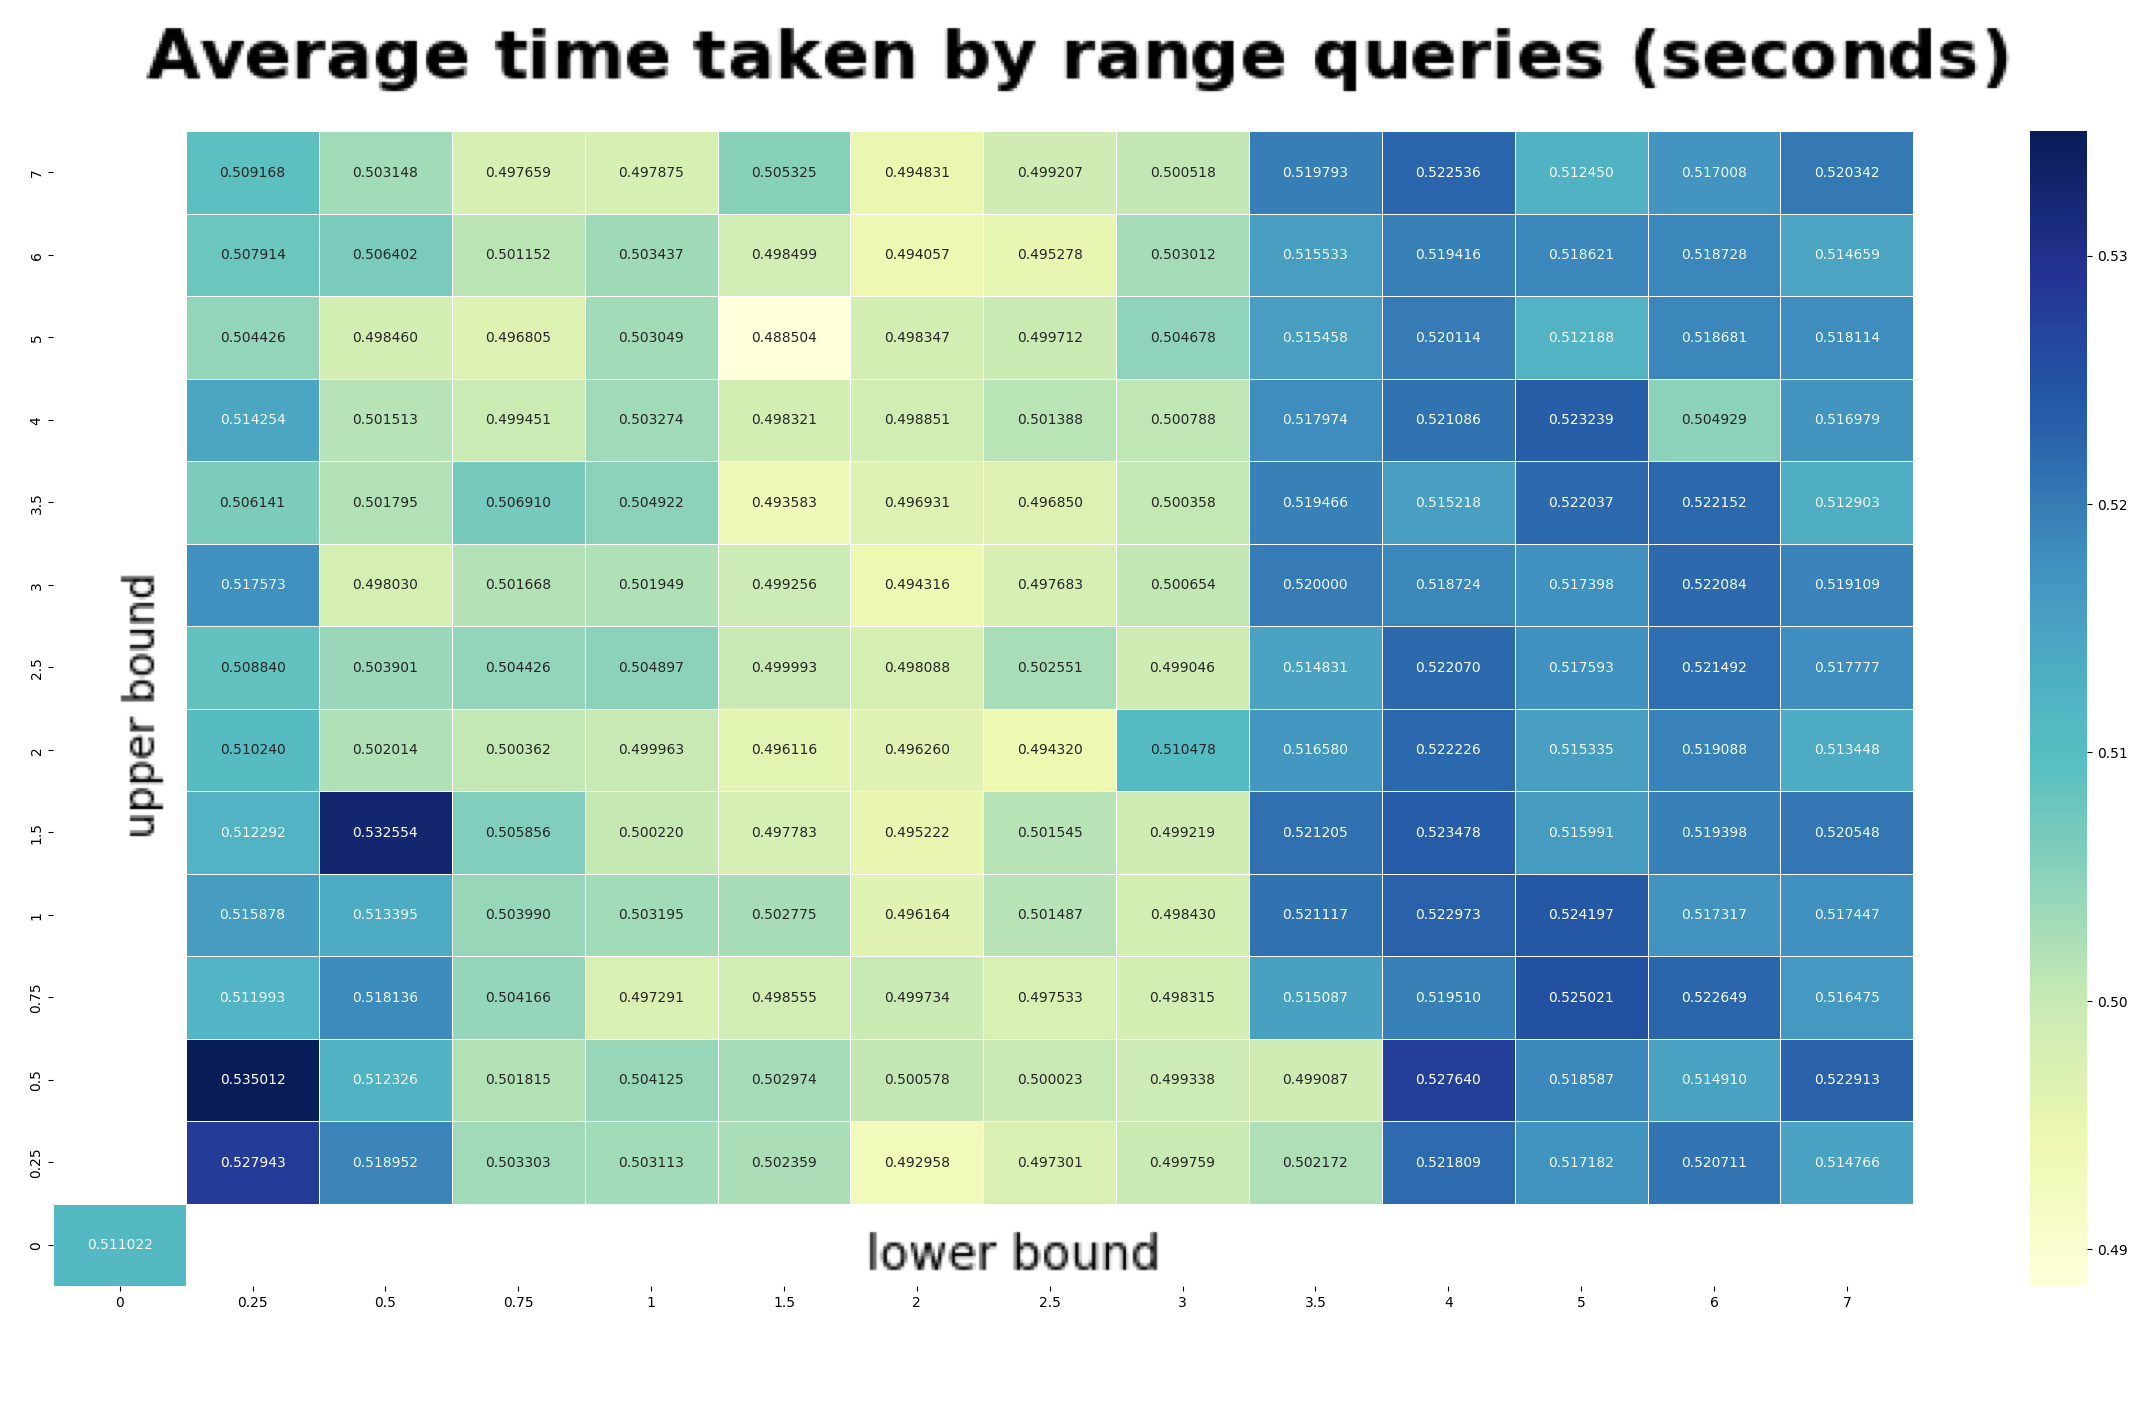
\includegraphics[width=\linewidth]{Figures/total_time_take_by_range_queries.png}
    \caption{Figure shows the change in average total time taken by range queries for different lower and upper bound 
    thresholds. The left bottom corner shows the Vanilla and rest all are for RQDC.}
\end{figure}

The results obtained thus far are highly promising, showcasing improvements in terms of space amplification, range query 
execution, and write amplification. This positive trend is particularly notable in the reduced space amplification 
coupled with enhanced range query performance, achieved with the same write amplification as the vanilla approach.

It's important to note that our experiments have primarily focused on updates. However, we anticipate that the inclusion 
of deletes, specifically in the form of point tombstones, will lead to a substantial reduction in write amplification. 
The Range Query Data Compaction (RQDC) approach, when encountering tombstones, effectively removes the corresponding 
entries from the tree, unless new updates occur after the insertion of the tombstone.

Our ongoing experiments aim to fine-tune and find more feasible values of \textit{lower\_bound} and \textit{upper\_bound}, 
recognizing that these values may vary for different size ratios and workloads. The trends observed so far, illustrated in 
Figure~\ref{fig:db_size_for_different_ub_lb} and Figure~\ref{fig:number_of_sst_files_ub_lb}, demonstrate changes in the 
size of the database with varying lower and upper bounds. Notably, the size ratio utilized in our experiments is 
randomly set at 6 \textit{(T)}.